\RequirePackage[l2tabu,orthodox]{nag}  % warn about common LaTeX pitfalls
\RequirePackage[ascii]{inputenc}  % input is 7-bit ASCII
\RequirePackage{fixltx2e}  % fix LaTeX2e kernel bugs

\documentclass[11pt,twoside]{article}
\usepackage{tikz}
\usepackage{tkz-graph}
\usepackage{pgfplots}
\usepackage{color}
\usepackage{calc}  % arithmetic in length parameters
\usepackage{enumitem}  % more control over list formatting
\usepackage{fancyhdr}  % simpler headers and footers
\usepackage[margin=1in]{geometry}  % page layout
\usepackage{lastpage}  % for last page number
\usepackage{relsize}  % easier font size changes
\usepackage[normalem]{ulem}  % smarter underlining
\usepackage{url}  % verb-like typesetting of URLs
%\usepackage{xfrac}  % nicer looking simple fractions for text and math
\usepackage{amsmath}
\usepackage{amssymb}

% Set up fonts.
\usepackage[T1]{fontenc}  % use true 8-bit fonts
\usepackage{slantsc}  % allow slanted small-caps
\usepackage{microtype}  % perform various font optimizations
% Use Palatino-based monospace instead of kpfonts' default.
%\usepackage{newpxtext}
\ttfamily
\DeclareFontShape{T1}{\ttdefault}{m}{scsl}{<->ssub*\ttdefault/m/sc}{}
\DeclareFontShape{T1}{\ttdefault}{b}{scsl}{<->ssub*\ttdefault/b/sc}{}
% "Kepler" fonts.
\usepackage[nott,notextcomp]{kpfonts}
% Use curvier Latin Modern brackets instead of kpfonts' glyphs.
\DeclareSymbolFont{lmsymb}     {OMS}{lmsy}{m}{n}
\DeclareSymbolFont{lmlargesymb}{OMX}{lmex}{m}{n}
\DeclareMathDelimiter{\rbrace}{\mathclose}{lmsymb}{"67}{lmlargesymb}{"09}
\DeclareMathDelimiter{\lbrace}{\mathopen}{lmsymb}{"66}{lmlargesymb}{"08}

% Page layout: stretch text to fill up page.
\addtolength\footskip{.25\headheight}
\flushbottom


% Headings.
\pagestyle{fancy}
\let\headrule\empty
\let\footrule\empty
\lhead{CSC\,418\,H1}
\chead{\large\scshape Assignment \#\,1}
\rhead{\scshape Fall 2015}
\cfoot{}
\rfoot{\scshape page \thepage\space of \pageref{LastPage}}


\begin{document}
\null\hfill \ \ \ \ \ \ \ \  Rui Ji (1000340918)
\begin{enumerate}
\item \begin{enumerate} [label=\roman*]
		\item To get tangent vector, we take derivative of $( x(t), y(t) )$ respect to $t$.\\
			$x'(t) =  (4 \cos(2 \pi t) + \frac{\cos(32 \pi t)}{ 16 })' = - 2\pi( 4\sin(2 \pi t) + \sin (32 \pi t))$ \\
			$y'(t) =  (2 \sin(2 \pi t) + \frac{\sin(32 \pi t)}{ 16 })' =  2\pi( 2\cos(2 \pi t) + \cos (32 \pi t))$\\
			Then the tangent vector is $(-(4\sin(2 \pi t) + \sin (32 \pi t)), ( 2\cos(2 \pi t) + \cos (32 \pi t)))$\
		\item To get normal vector, we know that at any point normal vector is perpendicular to tangent vector; hence,	
			normal vector is $(( 2\cos(2 \pi t) + \cos (32 \pi t)), (4\sin(2 \pi t) + \sin (32 \pi t)))$ or 
			$(- ( 2\cos(2 \pi t) + \cos (32 \pi t)), - (4\sin(2 \pi t) + \sin (32 \pi t)))$.
		\item The curve is symmetric around X-axis and symmetric around Y-axis. \\
			We could notice that both $x(t)$ and $y(t)$ are periodic functions which repeat over intervals of 1 radians. \\
			Also if a function $f(x)$ is symmetric around X-axis means $f(x) = - f(x)$ and is symmetric around Y-axis means $f(x) =  f(-x)$.\\
			Symmetric around X-axis:\\
			First, we know that $\cos(t) = \cos(-t)$ which means $x(t) = x(-t)$. Also, $\sin(t) = -\sin(-t)$ which means $y(t) = -y(-t)$.
			Then at $t$ and $-t$ time, the curve has same x coordinates but opposite y coordinates; hence, the curve is symmetric around X-axis.\\
			Symmetric around Y-axis:\\
			We know that $\cos(t) = - \cos(\pi-t)$ which means $x(t) = -x(0.5-t)$. Also, $\sin(t) = \sin(\pi-t)$ which means $y(t) = y(0.5-t)$.
			Then at $t$ and $0.5-t$ time, the curve has opposite x coordinates but same y coordinates; hence, the curve is symmetric around Y-axis.\\
		\item Since both $x(t)$ and $y(t)$ are periodic functions which repeat over intervals of 1radians, and symmetric around both X-axis and Y-axis.\\
			 Then  perimeter: \[p = 4 \int_{0}^{0.25} \sqrt{ (x'(t))^2 +( y'(t))^2} dt \]
			 			\[= 4\int_{0}^{0.25}  \sqrt{ (2\pi( 4\sin(2 \pi t) + \sin (32 \pi t)))^2 + (2\pi( 2\cos(2 \pi t) + \cos (32 \pi t)))^2 }dt  \]
		\item  Define $f(t)$ as follow:
		\[ f(t ) = \sqrt{ (2\pi( 4\sin(2 \pi t) + \sin (32 \pi t)))^2 + (2\pi( 2\cos(2 \pi t) + \cos (32 \pi t)))^2 }  \]
		The way we approximate the perimeter is approximate the integral above. So we divide the interval $ [0,0.25]$ to $n$ sub-interval $[x_0,x_1],[x_1,x_2] ...[x_{n-1}, x_{n}] \ where \ x_0 = 0, x_n = 0.25$. Then calculate sum, $perimeter = 4\sum_{i=0}^{i=n-1}[ (f(x_{i+1}) - f(x_i) )(x_{i+1} - x_i)]$.
	\end{enumerate}
	
	
\item Denote $C_1$ to be the circle with radius $r_1$ and $C_2$ to be the circle with radius $r_2 $ ($r_2 > r_1$).	
	\begin{enumerate} [label=\roman*]
		\item The area of donut is $A =\pi (r_2)^2 - \pi (r_1)^2 = \pi((r_2)^2- (r_1)^2)$.
		\item There can be 0,1, 2 ,3 and 4 intersections.
		\item The distance from the centre $(p_1)$ of the circles to line $p( \lambda ) = p_0 +\lambda \overrightarrow{d}$ is
			 \[distance: \ d =|| (p_0-p_1) -((p_0-p_1) \cdot \overrightarrow{n} ) \overrightarrow{n}}|| \ \ \ \ where \  \overrightarrow{n} = \frac {\overrightarrow{d}}{|\overrightarrow{d}|} \] 
			(1) if $d > r_2$, then there is no intersection; \\
			(2) if $d = r_2$, then there is 1 intersection, then solve the equation \[ || (p_0 - p_1) - \lambda \overrightarrow{d} ||  = r_2 \]   get one solution $ \lambda_0$ and $p( \lambda _0)$ is the location of the intersection.\\
			(3) if $r_2 > d > r_1$, then there 2 intersections, then solve the equation   \[ || (p_0 - p_1) - \lambda \overrightarrow{d} ||  = r_2 \]  get two solutions $ \lambda_0, \lambda_1$ and $p( \lambda _0), p( \lambda _1)$ are the location of the intersections.\\
			(4) if $ d = r_1$, then there are 3 intersections, then solve  then solve the equation   \[ || (p_0 - p_1) - \lambda \overrightarrow{d} ||  = r_2 \]   \[ || (p_0 - p_1) - \lambda \overrightarrow{d} ||  = r_1 \] get three solutions $ \lambda_0, \lambda_1 \lambda_2 $ and $p( \lambda _0), p( \lambda _1), p( \lambda _2)$ are the location of the intersections.\\
			(5) if $ d < r_1$, then there are 4 intersections, then solve  then solve the equation   \[ || (p_0 - p_1) - \lambda \overrightarrow{d} ||  = r_2 \]   \[ || (p_0 - p_1) - \lambda \overrightarrow{d} ||  = r_1 \] get three solutions $ \lambda_0, \lambda_1, \lambda_2,  \lambda_3 $ and $p( \lambda _0), p( \lambda _1), p( \lambda _2), p( \lambda _3)$ are the location of the intersections.
		\item If both line and donut transformed by a non-uniform scale $(s_x,s_y)$, then intersection won't change. Suppose the old location is $(x,y)$, then location after scale it will be $(s_xx,s_yy) $. 
		\item Suppose A$(x,y)$ is a point on the donut. After scaling, it becomes A' $(s_xx,s_yy)$. Then $\Delta(A'A) = (A'-A)$, and $\theta =\arccos( \frac{\overrightarrow{A'-A}\cdot\overrightarrow{d}}{|\overrightarrow{A'-A}| |\overrightarrow{d}|})$ . Then if $\pi < \theta < 2\pi$ means after scaling A is closer to the line, if  $0 < \theta < \pi$ means A is away from the line after scaling and $\theta = 0 \vee \theta = \pi$ means the distance from A to the line remains the same.
	\end{enumerate}

\item  \begin{itemize} [label={}] 
	\item (a) Translation and uniform scaling do not commute
			First, translate by $(1,0)$, then scaled by $(\frac{1}{2}, \frac{1}{2})$:
			\begin{center} 
			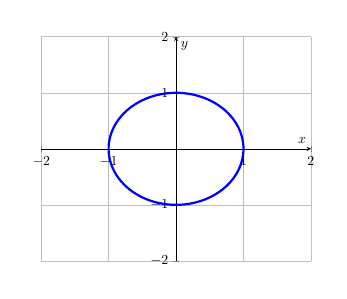
\begin{tikzpicture}[scale=0.5]
			\begin{axis}[
          			grid=both,
          			xmin=-2,
          			xmax=2,
          			ymin=-2,
          			ymax=2,
          			xlabel=$x$,
          			ylabel=$y$,
          			axis lines=center,
          			>=stealth
        				]
  			\addplot[
    				domain=0:2*pi,
    				blue,
    				ultra thick,
    				samples=100,
  				] plot[smooth] ( {cos(deg(x))},{sin(deg(x))});
			\end{axis}
			\end{tikzpicture}%
   			 ~%
    			%
			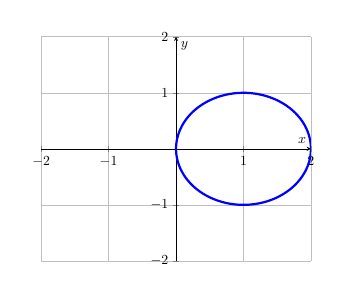
\begin{tikzpicture}[scale=0.5]
			\begin{axis}[
          			grid=both,
          			xmin=-2,
          			xmax=2,
          			ymin=-2,
          			ymax=2,
          			xlabel=$x$,
          			ylabel=$y$,
          			axis lines=center,
          			>=stealth
        				]
  			\addplot[
    				domain=0:2*pi,
    				blue,
    				ultra thick,
    				samples=100,
  				] plot[smooth] ( {cos(deg(x)) + 1},{sin(deg(x))});
			\end{axis}
			\end{tikzpicture}%
   			 ~%
    			%
			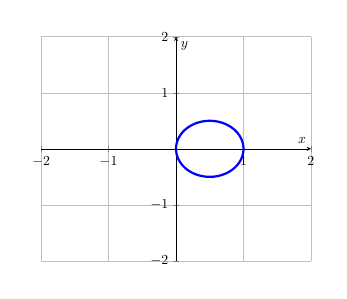
\begin{tikzpicture}[scale=0.5]
			\begin{axis}[
          			grid=both,
          			xmin=-2,
          			xmax=2,
          			ymin=-2,
          			ymax=2,
          			xlabel=$x$,
          			ylabel=$y$,
          			axis lines=center,
          			>=stealth
        				]
  			\addplot[
    				domain=0:2*pi,
    				blue,
    				ultra thick,
    				samples=100,
  				] plot[smooth] ( {(cos(deg(x)) + 1)/2},{(sin(deg(x)))/2});
			\end{axis}
			\end{tikzpicture}
			\end{center} 
			\\
			Now, apply it reversely, scaled by $(\frac{1}{2}, \frac{1}{2})$, then translate by $(1,0)$ :
			\begin{center} 
			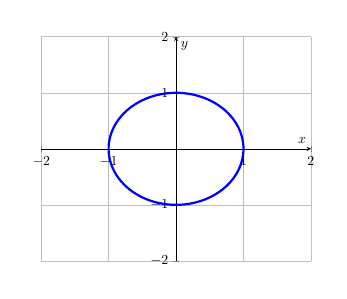
\begin{tikzpicture}[scale=0.5]
			\begin{axis}[
          			grid=both,
          			xmin=-2,
          			xmax=2,
          			ymin=-2,
          			ymax=2,
          			xlabel=$x$,
          			ylabel=$y$,
          			axis lines=center,
          			>=stealth
        				]
  			\addplot[
    				domain=0:2*pi,
    				blue,
    				ultra thick,
    				samples=100,
  				] plot[smooth] ( {cos(deg(x))},{sin(deg(x))});
			\end{axis}
			\end{tikzpicture}%
   			 ~%
    			%
			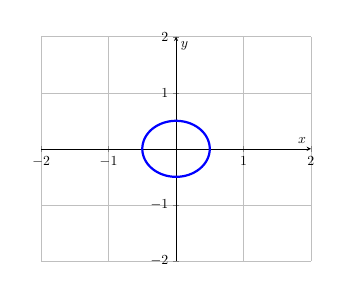
\begin{tikzpicture}[scale=0.5]
			\begin{axis}[
          			grid=both,
          			xmin=-2,
          			xmax=2,
          			ymin=-2,
          			ymax=2,
          			xlabel=$x$,
          			ylabel=$y$,
          			axis lines=center,
          			>=stealth
        				]
  			\addplot[
    				domain=0:2*pi,
    				blue,
    				ultra thick,
    				samples=100,
  				] plot[smooth] ( {(cos(deg(x)))/2},{(sin(deg(x)))/2});
			\end{axis}
			\end{tikzpicture}%
   			 ~%
    			%
			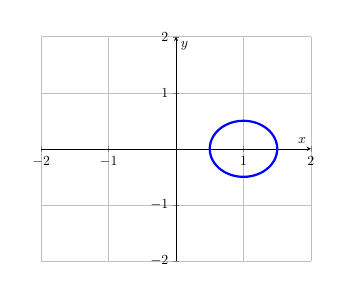
\begin{tikzpicture}[scale=0.5]
			\begin{axis}[
          			grid=both,
          			xmin=-2,
          			xmax=2,
          			ymin=-2,
          			ymax=2,
          			xlabel=$x$,
          			ylabel=$y$,
          			axis lines=center,
          			>=stealth
        				]
  			\addplot[
    				domain=0:2*pi,
    				blue,
    				ultra thick,
    				samples=100,
  				] plot[smooth] ( {(cos(deg(x)))/2 + 1},{(sin(deg(x)))/2});
			\end{axis}
			\end{tikzpicture}
			\end{center} 
			Hence, clearly translation and uniform scaling do not commute.
	\item (b) Translation and non-uniform scaling do not commute.
			First we scaled by $(1, \frac{1}{2})$, then translate by $(0,1)$ :
			\begin{center} 
			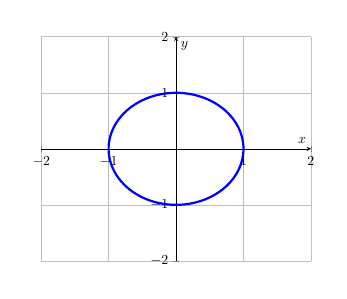
\begin{tikzpicture}[scale=0.5]
			\begin{axis}[
          			grid=both,
          			xmin=-2,
          			xmax=2,
          			ymin=-2,
          			ymax=2,
          			xlabel=$x$,
          			ylabel=$y$,
          			axis lines=center,
          			>=stealth
        				]
  			\addplot[
    				domain=0:2*pi,
    				blue,
    				ultra thick,
    				samples=100,
  				] plot[smooth] ( {cos(deg(x))},{sin(deg(x))});
			\end{axis}
			\end{tikzpicture}%
   			 ~%
    			%
			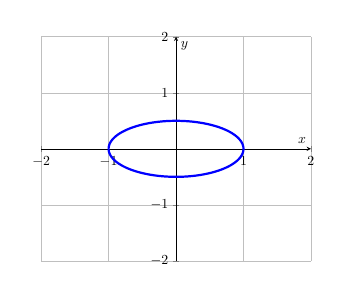
\begin{tikzpicture}[scale=0.5]
			\begin{axis}[
          			grid=both,
          			xmin=-2,
          			xmax=2,
          			ymin=-2,
          			ymax=2,
          			xlabel=$x$,
          			ylabel=$y$,
          			axis lines=center,
          			>=stealth
        				]
  			\addplot[
    				domain=0:2*pi,
    				blue,
    				ultra thick,
    				samples=100,
  				] plot[smooth] ( {(cos(deg(x)))},{(sin(deg(x)))/2});
			\end{axis}
			\end{tikzpicture}%
   			 ~%
    			%
			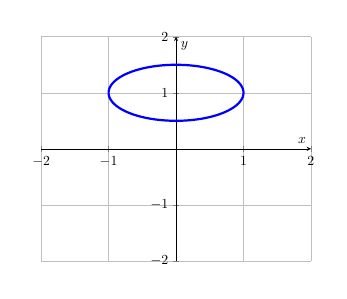
\begin{tikzpicture}[scale=0.5]
			\begin{axis}[
          			grid=both,
          			xmin=-2,
          			xmax=2,
          			ymin=-2,
          			ymax=2,
          			xlabel=$x$,
          			ylabel=$y$,
          			axis lines=center,
          			>=stealth
        				]
  			\addplot[
    				domain=0:2*pi,
    				blue,
    				ultra thick,
    				samples=100,
  				] plot[smooth] ( {(cos(deg(x)))},{(sin(deg(x)))/2 + 1});
			\end{axis}
			\end{tikzpicture}
			\end{center} 
			Now, we apply translation first, then scaling:
			\begin{center} 
			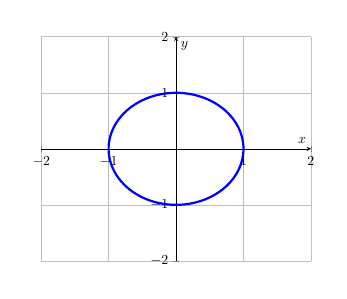
\begin{tikzpicture}[scale=0.5]
			\begin{axis}[
          			grid=both,
          			xmin=-2,
          			xmax=2,
          			ymin=-2,
          			ymax=2,
          			xlabel=$x$,
          			ylabel=$y$,
          			axis lines=center,
          			>=stealth
        				]
  			\addplot[
    				domain=0:2*pi,
    				blue,
    				ultra thick,
    				samples=100,
  				] plot[smooth] ( {cos(deg(x))},{sin(deg(x))});
			\end{axis}
			\end{tikzpicture}%
   			 ~%
    			%
			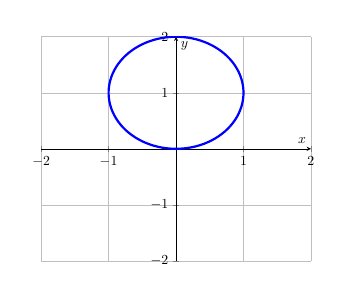
\begin{tikzpicture}[scale=0.5]
			\begin{axis}[
          			grid=both,
          			xmin=-2,
          			xmax=2,
          			ymin=-2,
          			ymax=2,
          			xlabel=$x$,
          			ylabel=$y$,
          			axis lines=center,
          			>=stealth
        				]
  			\addplot[
    				domain=0:2*pi,
    				blue,
    				ultra thick,
    				samples=100,
  				] plot[smooth] ( {(cos(deg(x)))},{(sin(deg(x))) + 1});
			\end{axis}
			\end{tikzpicture}%
   			 ~%
    			%
			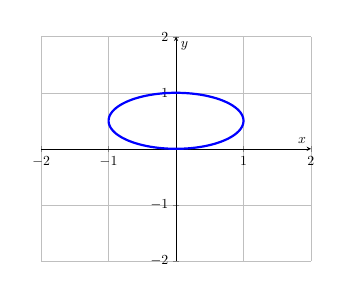
\begin{tikzpicture}[scale=0.5]
			\begin{axis}[
          			grid=both,
          			xmin=-2,
          			xmax=2,
          			ymin=-2,
          			ymax=2,
          			xlabel=$x$,
          			ylabel=$y$,
          			axis lines=center,
          			>=stealth
        				]
  			\addplot[
    				domain=0:2*pi,
    				blue,
    				ultra thick,
    				samples=100,
  				] plot[smooth] ( {(cos(deg(x)))},{(sin(deg(x))+1)/2});
			\end{axis}
			\end{tikzpicture}
			\end{center} 
			Hence, translation and non-uniform scaling do not commute.
	\item (c) Scaling and rotation, both having the same fixed points commute.\\
		Scaling by $(1,2)$, then rotating $\frac{\pi}{2}$:
		\begin{center} 
			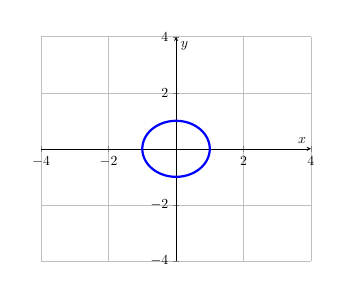
\begin{tikzpicture}[scale=0.5]
			\begin{axis}[
          			grid=both,
          			xmin=-4,
          			xmax=4,
          			ymin=-4,
          			ymax=4,
          			xlabel=$x$,
          			ylabel=$y$,
          			axis lines=center,
          			>=stealth
        				]
  			\addplot[
    				domain=0:2*pi,
    				blue,
    				ultra thick,
    				samples=100,
  				] plot[smooth] ( {cos(deg(x))},{sin(deg(x))});
			\end{axis}
			\end{tikzpicture}%
   			 ~%
    			%
			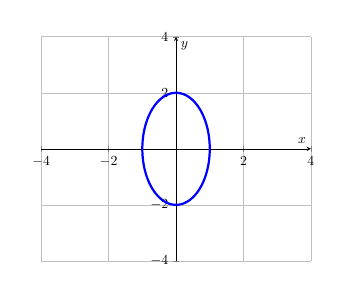
\begin{tikzpicture}[scale=0.5]
			\begin{axis}[
          			grid=both,
          			xmin=-4,
          			xmax=4,
          			ymin=-4,
          			ymax=4,
          			xlabel=$x$,
          			ylabel=$y$,
          			axis lines=center,
          			>=stealth
        				]
  			\addplot[
    				domain=0:2*pi,
    				blue,
    				ultra thick,
    				samples=100,
  				] plot[smooth] ( {cos(deg(x))},{2*(sin(deg(x))});
			\end{axis}
			\end{tikzpicture}%
   			 ~%
    			%
			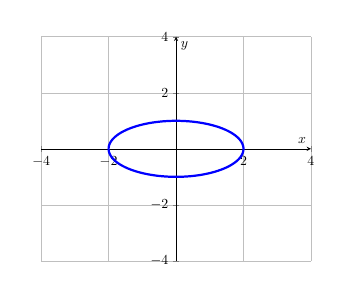
\begin{tikzpicture}[scale=0.5]
			\begin{axis}[
          			grid=both,
          			xmin=-4,
          			xmax=4,
          			ymin=-4,
          			ymax=4,
          			xlabel=$x$,
          			ylabel=$y$,
          			axis lines=center,
          			>=stealth
        				]
  			\addplot[
    				domain=0:2*pi,
    				blue,
    				ultra thick,
    				samples=100,
  				] plot[smooth] ( {-2*(sin(deg(x))},{cos(deg(x))});
			\end{axis}
			\end{tikzpicture}
			\end{center} 
			
			Now, rotating first then scaling
			\begin{center} 
			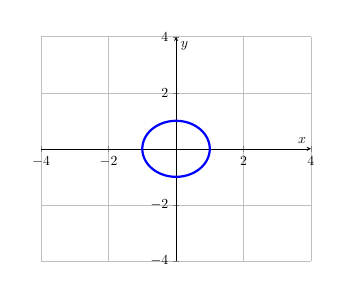
\begin{tikzpicture}[scale=0.5]
			\begin{axis}[
          			grid=both,
          			xmin=-4,
          			xmax=4,
          			ymin=-4,
          			ymax=4,
          			xlabel=$x$,
          			ylabel=$y$,
          			axis lines=center,
          			>=stealth
        				]
  			\addplot[
    				domain=0:2*pi,
    				blue,
    				ultra thick,
    				samples=100,
  				] plot[smooth] ( {cos(deg(x))},{sin(deg(x))});
			\end{axis}
			\end{tikzpicture}%
   			 ~%
    			%
			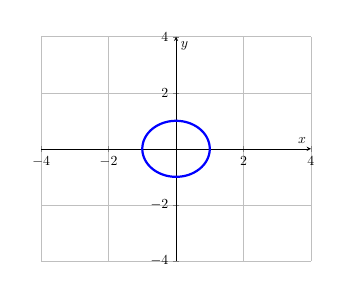
\begin{tikzpicture}[scale=0.5]
			\begin{axis}[
          			grid=both,
          			xmin=-4,
          			xmax=4,
          			ymin=-4,
          			ymax=4,
          			xlabel=$x$,
          			ylabel=$y$,
          			axis lines=center,
          			>=stealth
        				]
  			\addplot[
    				domain=0:2*pi,
    				blue,
    				ultra thick,
    				samples=100,
  				] plot[smooth] ( {(sin(deg(x))},{cos(deg(x))});
			\end{axis}
			\end{tikzpicture}%
   			 ~%
    			%
			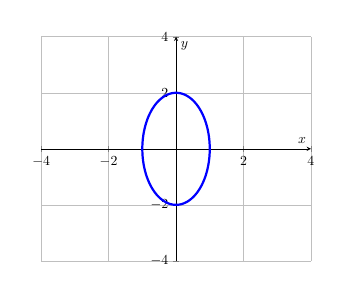
\begin{tikzpicture}[scale=0.5]
			\begin{axis}[
          			grid=both,
          			xmin=-4,
          			xmax=4,
          			ymin=-4,
          			ymax=4,
          			xlabel=$x$,
          			ylabel=$y$,
          			axis lines=center,
          			>=stealth
        				]
  			\addplot[
    				domain=0:2*pi,
    				blue,
    				ultra thick,
    				samples=100,
  				] plot[smooth]  ( {(sin(deg(x))},{2*cos(deg(x))});
			\end{axis}
			\end{tikzpicture}
			\end{center} 
	\item (d) Scaling and scaling, having different fixed points do not commute.
	First, Scaling around $(0,0)$ by (2,0), then around $(1, 0)$ by (2, 0):
		\begin{center} 
			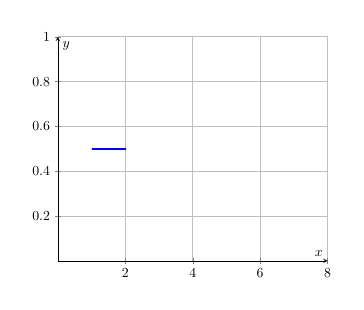
\begin{tikzpicture}[scale=0.5]
			\begin{axis}[
          			grid=both,
          			xmin=0,
          			xmax=8,
          			ymin=0,
          			ymax=1,        			
				xlabel=$x$,
          			ylabel=$y$,
          			axis lines=center,
          			>=stealth
        				]
  			\addplot[
    				domain=1:2,
    				blue,
    				ultra thick,
    				samples=100,
  				] plot[smooth] ( {x},{0.5});
			\end{axis}
			\end{tikzpicture}%
   			 ~%
    			%
			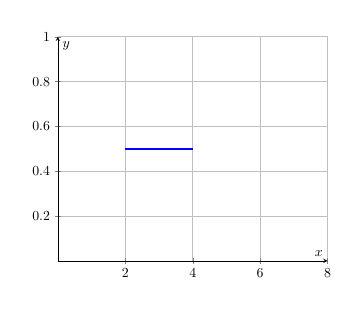
\begin{tikzpicture}[scale=0.5]
			\begin{axis}[
          			grid=both,
          			xmin=0,
          			xmax=8,
          			ymin=0,
          			ymax=1,
          			xlabel=$x$,
          			ylabel=$y$,
          			axis lines=center,
          			>=stealth
        				]
  			\addplot[
    				domain=1:2,
    				blue,
    				ultra thick,
    				samples=100,
  				] plot[smooth] ({2*x},{0.5});
			\end{axis}
			\end{tikzpicture}%
   			 ~%
    			%
			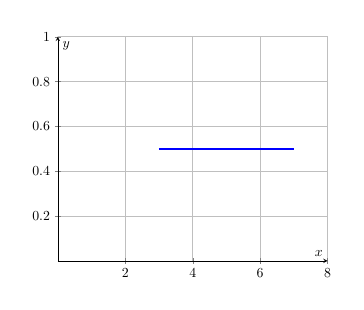
\begin{tikzpicture}[scale=0.5]
			\begin{axis}[
          			grid=both,
          			xmin=0,
          			xmax=8,
          			ymin=0,
          			ymax=1,
          			xlabel=$x$,
          			ylabel=$y$,
          			axis lines=center,
          			>=stealth
        				]
  			\addplot[
    				domain=1:2,
    				blue,
    				ultra thick,
    				samples=100,
  				] plot[smooth] ({4*x-1},{0.5});
			\end{axis}
			\end{tikzpicture}
			\end{center} 
			First, Scaling around $(1, 0)$ by (2, 0),  then around $(0,0)$ by (2,0) :
		\begin{center} 
			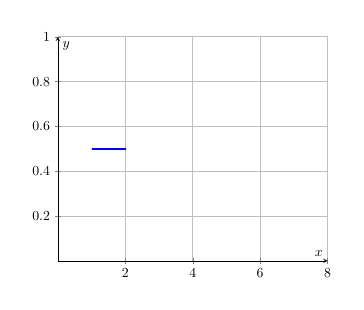
\begin{tikzpicture}[scale=0.5]
			\begin{axis}[
          			grid=both,
          			xmin=0,
          			xmax=8,
          			ymin=0,
          			ymax=1,
          			xlabel=$x$,
          			ylabel=$y$,
          			axis lines=center,
          			>=stealth
        				]
  			\addplot[
    				domain=1:2,
    				blue,
    				ultra thick,
    				samples=100,
  				] plot[smooth] ( {x},{0.5});
			\end{axis}
			\end{tikzpicture}%
   			 ~%
    			%
			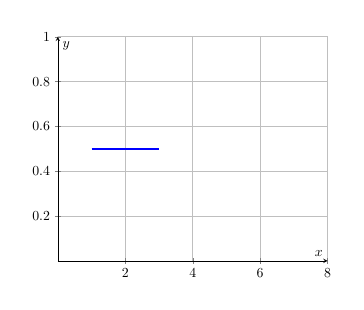
\begin{tikzpicture}[scale=0.5]
			\begin{axis}[
          			grid=both,
          			xmin=0,
          			xmax=8,
          			ymin=0,
          			ymax=1,
          			xlabel=$x$,
          			ylabel=$y$,
          			axis lines=center,
          			>=stealth
        				]
  			\addplot[
    				domain=1:2,
    				blue,
    				ultra thick,
    				samples=100,
  				] plot[smooth] ( {2*x-1},{0.5});
			\end{axis}
			\end{tikzpicture}%
   			 ~%
    			%
			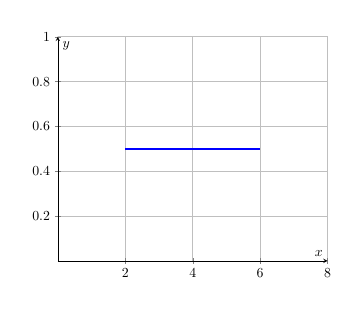
\begin{tikzpicture}[scale=0.5]
			\begin{axis}[
          			grid=both,
          			xmin=0,
          			xmax=8,
          			ymin=0,
          			ymax=1,
          			xlabel=$x$,
          			ylabel=$y$,
          			axis lines=center,
          			>=stealth
        				]
  			\addplot[
    				domain=1:2,
    				blue,
    				ultra thick,
    				samples=100,
  				] plot[smooth] ( {4*x-2},{0.5});
			\end{axis}
			\end{tikzpicture}
		\end{center} 

	\item (e) Translation and shear do not commute.
		First, shearing by $  \begin{bmatrix} 1 & 2  \\ 0 & 1  \end{bmatrix}$, then  translate by $(0,1)$:
		\begin{center} 
			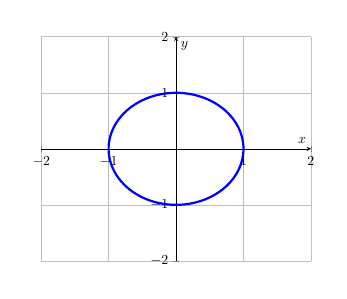
\begin{tikzpicture}[scale=0.5]
			\begin{axis}[
          			grid=both,
          			xmin=-2,
          			xmax=2,
          			ymin=-2,
          			ymax=2,
          			xlabel=$x$,
          			ylabel=$y$,
          			axis lines=center,
          			>=stealth
        				]
  			\addplot[
    				domain=0:2*pi,
    				blue,
    				ultra thick,
    				samples=100,
  				] plot[smooth] ( {cos(deg(x))},{sin(deg(x))});
			\end{axis}
			\end{tikzpicture}%
   			 ~%
    			%
			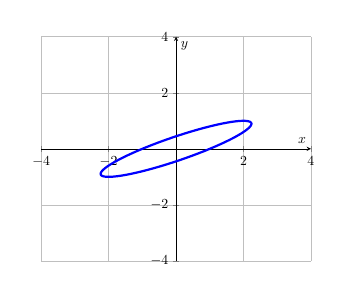
\begin{tikzpicture}[scale=0.5]
			\begin{axis}[
          			grid=both,
          			xmin=-4,
          			xmax=4,
          			ymin=-4,
          			ymax=4,
          			xlabel=$x$,
          			ylabel=$y$,
          			axis lines=center,
          			>=stealth
        				]
  			\addplot[
    				domain=0:2*pi,
    				blue,
    				ultra thick,
    				samples=100,
  				] plot[smooth] ( {(cos(deg(x)) + 2*sin(deg(x))},{sin(deg(x)});
			\end{axis}
			\end{tikzpicture}%
   			 ~%
    			%
			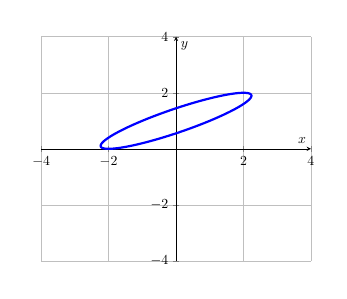
\begin{tikzpicture}[scale=0.5]
			\begin{axis}[
          			grid=both,
          			xmin=-4,
          			xmax=4,
          			ymin=-4,
          			ymax=4,
          			xlabel=$x$,
          			ylabel=$y$,
          			axis lines=center,
          			>=stealth
        				]
  			\addplot[
    				domain=0:2*pi,
    				blue,
    				ultra thick,
    				samples=100,
  				] plot[smooth] ( {(cos(deg(x)) + 2*sin(deg(x))},{sin(deg(x))+1});
			\end{axis}
			\end{tikzpicture}
			\end{center} 
			Now, we first translate by $(0,1)$ then shearing by $  \begin{bmatrix} 1 & 2  \\ 0 & 1  \end{bmatrix}$:
		\begin{center} 
			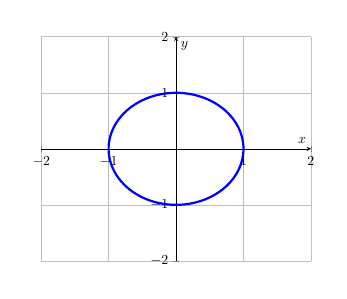
\begin{tikzpicture}[scale=0.5]
			\begin{axis}[
          			grid=both,
          			xmin=-2,
          			xmax=2,
          			ymin=-2,
          			ymax=2,
          			xlabel=$x$,
          			ylabel=$y$,
          			axis lines=center,
          			>=stealth
        				]
  			\addplot[
    				domain=0:2*pi,
    				blue,
    				ultra thick,
    				samples=100,
  				] plot[smooth] ( {cos(deg(x))},{sin(deg(x))});
			\end{axis}
			\end{tikzpicture}%
   			 ~%
    			%
			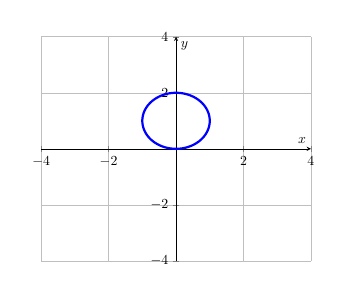
\begin{tikzpicture}[scale=0.5]
			\begin{axis}[
          			grid=both,
          			xmin=-4,
          			xmax=4,
          			ymin=-4,
          			ymax=4,
          			xlabel=$x$,
          			ylabel=$y$,
          			axis lines=center,
          			>=stealth
        				]
  			\addplot[
    				domain=0:2*pi,
    				blue,
    				ultra thick,
    				samples=100,
  				] plot[smooth] ( {cos(deg(x))},{sin(deg(x))+1});
			\end{axis}
			\end{tikzpicture}%
   			 ~%
    			%
			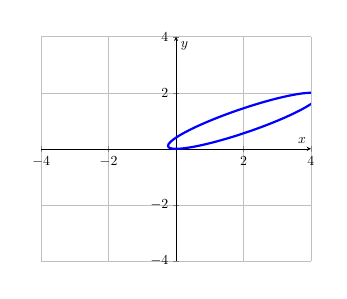
\begin{tikzpicture}[scale=0.5]
			\begin{axis}[
          			grid=both,
          			xmin=-4,
          			xmax=4,
          			ymin=-4,
          			ymax=4,
          			xlabel=$x$,
          			ylabel=$y$,
          			axis lines=center,
          			>=stealth
        				]
  			\addplot[
    				domain=0:2*pi,
    				blue,
    				ultra thick,
    				samples=100,
  				] plot[smooth] ( {cos(deg(x)) + 2*(sin(deg(x))+1)},{sin(deg(x))+1});
			\end{axis}
			\end{tikzpicture}
		\end{center} 
		Hence, translation and shear do not commute.
	\end{itemize}
\item \begin{enumerate} [label=\roman*]
		\item  First we create 3 vectors $\overrightarrow {v_0-q},\overrightarrow {v_1-q}, \overrightarrow {v_2-q}$ using $\bar{v_0}, \bar{v_1} , \bar{v_2}$ and $\bar{q}$. 
				\[\theta_0 = \arccos(\frac{\overrightarrow {v_0-q} \cdot \overrightarrow {v_1-q}}{|\overrightarrow {v_0-q}||\overrightarrow {v_1-q}|} )\] 
				\[\theta_1 = \arccos(\frac{\overrightarrow {v_0-q} \cdot \overrightarrow {v_2-q}}{|\overrightarrow {v_0-q}||\overrightarrow {v_2-q}|}) \]
				\[ \theta_2 = \arccos(\frac{\overrightarrow {v_1-q} \cdot \overrightarrow {v_2-q}}{|\overrightarrow {v_1-q}||\overrightarrow {v_2-q}|})\]
			Then $q$ is inside the triangle iff $(\theta_0 + \theta_1 + \theta_2= 2\pi) \wedge (\theta_0 \neq \pi) \wedge (\theta_1 \neq \pi)\wedge (\theta_2 \neq \pi)$;\\
	  		$q$ is on the triangle iff $ ( \ (v_0 = q) \vee (v_1 =q) \vee (v_2 = q) \ ) \  \vee \ ( \ (\theta_0 + \theta_1 + \theta_2= 2\pi) \wedge ((\theta_0 = \pi) \vee (\theta_1 = \pi)\vee (\theta_2 = \pi) ) \ )$;\\
	  		Otherwise, $q$ is outside the triangle.\\
		\item  Suppose we are given with 4 vertices $V= \{v_0, v_1, v_2, v_3\}$ and edge set $E = \{(v_0, v_1), (v_1, v_2),(v_2,v_3), (v_3, v_0)\}$.\\
                        	\begin{itemize} [label={}]
				\item  Define: \[\theta_0 = \arccos(\frac{\overrightarrow {v_1-v_0} \cdot \overrightarrow {v_2-v_0}}{|\overrightarrow {v_1-v_0}||\overrightarrow {v_2-v_0}|})+ \arccos(\frac{\overrightarrow {v_1-v_0} \cdot \overrightarrow {v_3-v_0}}{|\overrightarrow {v_1-v_0}||\overrightarrow {v_3-v_0}|}) + \arccos(\frac{\overrightarrow {v_2-v_0} \cdot \overrightarrow {v_3-v_0}}{|\overrightarrow {v_2-v_0}||\overrightarrow {v_3-v_0}|})\] 
						 \[\theta_1 = \arccos(\frac{\overrightarrow {v_0-v_1} \cdot \overrightarrow {v_2-v_1}}{|\overrightarrow {v_0-v_1}||\overrightarrow {v_2-v_1}|})+ \arccos(\frac{\overrightarrow {v_0-v_1} \cdot \overrightarrow {v_3-v_1}}{|\overrightarrow {v_0-v_1}||\overrightarrow {v_3-v_1}|}) + \arccos(\frac{\overrightarrow {v_2-v_1} \cdot \overrightarrow {v_3-v_1}}{|\overrightarrow {v_2-v_1}||\overrightarrow {v_3-v_1}|})\] 
						 \[\theta_2 = \arccos(\frac{\overrightarrow {v_1-v_2} \cdot \overrightarrow {v_3-v_2}}{|\overrightarrow {v_1-v_2}||\overrightarrow {v_3-v_2}|})+ \arccos(\frac{\overrightarrow {v_1-v_2} \cdot \overrightarrow {v_0-v_2}}{|\overrightarrow {v_1-v_2}||\overrightarrow {v_0-v_2}|}) + \arccos(\frac{\overrightarrow {v_0-v_2} \cdot \overrightarrow {v_3-v_2}}{|\overrightarrow {v_0-v_2}||\overrightarrow {v_3-v_2}|})\] 
						 \[\theta_3 = \arccos(\frac{\overrightarrow {v_1-v_3} \cdot \overrightarrow {v_2-v_3}}{|\overrightarrow {v_1-v_3}||\overrightarrow {v_2-v_3}|})+ \arccos(\frac{\overrightarrow {v_1-v_3} \cdot \overrightarrow {v_0-v_3}}{|\overrightarrow {v_1-v_3}||\overrightarrow {v_0-v_3}|}) + \arccos(\frac{\overrightarrow {v_0-v_3} \cdot \overrightarrow {v_2-v_3}}{|\overrightarrow {v_0-v_3}||\overrightarrow {v_2-v_3}|})\] 
				\item Check  if any $\theta_0 , \theta_1 , \theta_2 , \theta_3$  equals $2\pi$, if $\theta_x = 2\pi$ we know that quadrilateral is concave. And based on (i) we also know that $v_x$ is inside the triangle with vertices $V\setminus v_x$. Then connect $v_x, v_y$ where $(v_y \in V\setminus v_x) \wedge( (v_x,v_y) \notin E)$, and quadrilateral is now split into the union of two triangles.
					\item If none of $\theta_0 , \theta_1 , \theta_2 , \theta_3$ equals $2\pi$ which means the quadrilateral is convex. Then just connect one of two diagonals (i.e $(v_0, v_2)$ or $(v_1,v_3)$), the quadrilateral is now split into the union of two triangles.
                        		\end{itemize}
		\item  Suppose we are given with n vertices $V= \{v_0, v_1, v_2, v_3 ... v_(n-1)\}$ and edge set 
				$E = \{(v_0, v_1), (v_1, v_2),(v_2,v_3), (v_3, v_4) ... ,(v_{n-2}, v_{n-1}), (v_{n-1}, v_0)\}$.
				pick any vertex $v_i$ in the vertices set $V$ (i.e $v_0$), then connect $v_i$ to the rest of the vertices if there no edge between them.
		\item	Counterexample, this algorithm won't work for concave, for example  if we choose  $v_i = v_2$ in the following graph.
				\begin{center}
				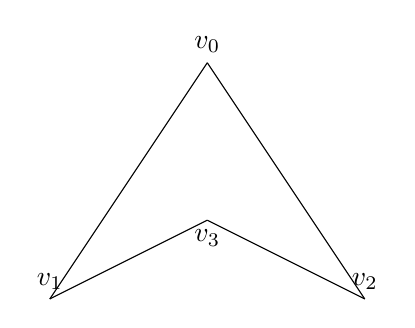
\begin{tikzpicture}[x=2cm,y=1cm]
                                     	\draw (0,2) node[anchor=south] {$v_0$};
					\draw (-1,-1) node[anchor=south] {$v_1$};
					\draw (1,-1) node[anchor=south] {$v_2$};
					\draw (0,0) node[anchor=north] {$v_3$};
					\draw[-] (0,2)--(-1,-1);
					\draw[-] (0,2)--(1,-1);
					\draw[-] (-1,-1)--(0,0);
					\draw[-] (1,-1)--(0,0);
                                 \end{tikzpicture}%
                                 ~%
                                 % 
                                 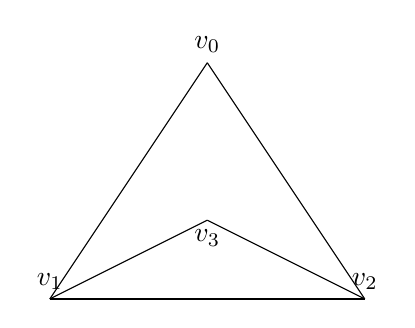
\begin{tikzpicture}[x=2cm,y=1cm]
                                     	\draw (0,2) node[anchor=south] {$v_0$};
					\draw (-1,-1) node[anchor=south] {$v_1$};
					\draw (1,-1) node[anchor=south] {$v_2$};
					\draw (0,0) node[anchor=north] {$v_3$};
					\draw[-] (0,2)--(-1,-1);
					\draw[-] (0,2)--(1,-1);
					\draw[-] (-1,-1)--(0,0);
					\draw[-] (1,-1)--(0,0);
					\draw[-] (1,-1)--(-1,-1);
                                 \end{tikzpicture}
                                 \end{center}
				
		\item For any point $q$, we connect $q$ with every vertex in the vertices set $V$, and define
				\[\theta_i = \arccos(\frac{ \overrightarrow {v_i-q} \cdot \overrightarrow {v_{i+1}_{(mod \ n)}-q} }{|\overrightarrow {v_i-q}||\overrightarrow {v_{i+1}_{(mod \ n)}-q}|} ) \ \ \ 0 \leq i \leq n-1 \] 
			
			Also, define the line function for each edge $i$ is $l_i$. Then $q$ is inside the polygon iff $\sum_{i=0}^{n-1}  \theta_i= 2\pi$ and $q$ doesn't satisfy any line function $l_i$. $q$ is on the polygon iff $\sum_{i=0}^{n-1}  \theta_i= 2\pi$ and satisfy some line function $l_i$. Otherwise, $q$ is outside the polygon.
	\end{enumerate}
\end{enumerate}

\end{document}
